\chapter{Постановка задачи}

\section{Описание задачи}

Создать таблицу, содержащую не менее 40 записей с вариантной частью. Произвести 
поиск  информации  по  вариантному  полю.  Упорядочить  таблицу,  по  возрастанию  ключей 
(где  ключ  –  любое  невариантное  поле  по  выбору  программиста),  используя:  а)  исходную 
таблицу;  б) массив  ключей, используя  2  разных  алгоритма сортировки  (простой, 
ускоренный).  Оценить  эффективность  этих  алгоритмов  (по  времени  и  по  используемому 
объему памяти) при различной реализации программы, то есть, в случаях а) и б). Обосновать 
выбор алгоритмов сортировки. Оценка эффективности должна быть относительной (в \%).

\section{Техническое задание}

Имеются описания: 
Type   жилье = (дом, общежитие); 
Данные:  
Фамилия, имя, группа, пол (м, ж), возраст, средний 
балл за сессию, дата поступления 
адрес:  
дом: (улица, No. дома, No. кв); 
общежитие: (No. общ., No. комн.); 

Ввести общий список студентов. 
Вывести список студентов, указанного года поступления, 
живущих в общежитии.

\paragraph{Сортировки: }

В данной лабораторной работе для упорядочивания таблицы будут применены следующие алгоритмы:

\begin{itemize}
	\item Сортировка выбором (Selection sort) -- временная сложность $O(n^2)$
	\item Сортировка слиянием (Merge sort) -- временная сложность $O(nlogn)$
\end{itemize}

\chapter{Конструкторский раздел}

В данном разделе представлены листинги кодов используемых структур данных.

\section{Описание Структур Данных}

В листингах 2.1 - 2.7 приведены используемые в программе структуры данных. Применение типа <<запись>> с вариантной частью обоснована тем, что при хранении информации о месте проживания студента, целесообразно хранить либо информацию об общежитии, либо информацию о квартире.  

\begin{lstlisting}[language=C,caption=Структура Таблицы]
typedef struct studtable
{
	student_t* data;
	unsigned int size;
} studtable_t;
\end{lstlisting}

\begin{lstlisting}[language=C,caption=Структура таблицы ключей]
typedef struct keytable
{
	_key_t* data;
	size_t size;
} keytable_t;
\end{lstlisting}

\begin{lstlisting}[language=C,caption=Структура ключа]
typedef struct key
{
	size_t id;
	double avg;
} _key_t;
\end{lstlisting}

\begin{lstlisting}[language=C,caption=Структура студента]
typedef struct
{
	char surname[MAX_STR];
	char name[MAX_STR];
	char group[MAX_STR];
	gender_t gender;
	uint16_t age;
	double avg_score;
	date_t enroll_date;
	housing_t house;
	union housing
	{
		dorm_t dorm;
		appartment_t appartment;
	} housing;
} student_t;
\end{lstlisting}

\begin{lstlisting}[language=C,caption=Перечисляемый тип пола]
typedef enum
{
	UNDEFINED,
	MALE,
	FEMALE
} gender_t;
\end{lstlisting}

\begin{lstlisting}[language=C,caption=Структура даты]
typedef struct
{
	uint16_t year;
	uint16_t month;
	uint16_t day;
} date_t;
\end{lstlisting}

\begin{lstlisting}[language=C,caption=Перечисляемый тип жилья]
typedef enum
{
	UNKNOWN,
	DORM,
	APPARTMENT
} housing_t;
\end{lstlisting}

\chapter{Технологический раздел}

\section{Требование к ПО}

\paragraph{Требования ко вводу: }

\begin{enumerate}
	\item На вход программе подается пункт меню (число от 0 до 9).
	\item На вход подается файл с данными студентов в заданном формате: \\
	\textit{<Фамилия>;<Имя>;<Группа>;<Пол>;<Возраст>;<Средний балл>;<Дата поступления>;<Где проживает>;[...];} В зависимости от поля \textit{<где проживает> [...]:} \\
	\textbf{dorm} : \textit{<номер общежития>,<номер комнаты>;} \\
	\textbf{appartment} : \textit{<улица>,<дом>,<квартира>;}
	\item ПО должно:
	\begin{itemize}
		\item Выводить таблицу студентов.
		\item Выводить список студентов указанного года поступления, живущих в общежитии.
		\item Сортировать исходную таблицу.
		\item Выводить таблицу ключей.
		\item Сортировать таблицу ключей.
		\item Выводить отсортированную исходную таблицу по таблице ключей.
		\item Добавлять студентов в таблицу (ввод с клавиатуры).
		\item Удалять студентов из таблицы по ключу (id).
		\item Проводить анализ временной сложности алгоритмов сортировки.
	\end{itemize}
	\item ПО должно выводить потраченную память и время.
\end{enumerate}

\section{Возможные аварийные ситуации}
\begin{itemize}
	\item Некорректный ввод данных.
	\item Пустой файл.
\end{itemize}

\section{Реализация алгоритмов}

В листингах \ref{aux}, \ref{merge} представлены вспомогательные функции для сортировок.

В листингах \ref{selection_sort}, \ref{merge_sort} представлены реализации алгоритмов сортировки Выбором и Слиянием.

\begin{lstlisting}[label=aux,language=C,caption=Вспомогательные функции]
static void swap(void* a, void* b, size_t size)
{
	for (size_t i = 0; i < size; i++)
	{
		*((char*)a + i) ^= *((char*)b + i);
		*((char*)b + i) ^= *((char*)a + i);
		*((char*)a + i) ^= *((char*)b + i);
	}
}

static size_t min_index(const void* base, size_t nitems, size_t size, compare_t cmp)
{
	size_t res = 0;
	const void* min_el = base;
	
	for (size_t i = 1; i < nitems; i++)
	{
		const void* elem = (const char*)base + i * size;
		if (cmp(elem, min_el) < 0)
		{
			min_el = elem;
			res = i;
		}
	}
	
	return res;
}
\end{lstlisting}

\begin{lstlisting}[label=selection_sort,language=C,caption=Сортировка выбором]
void selection_sort(void* base, size_t nitems, size_t size, compare_t cmp)
{
	for (size_t i = 0; i < nitems; i++)
	{
		size_t min_i = min_index((char*)base + i * size, nitems - i, size, cmp);
		if (min_i != 0)
			swap((char*)base + i * size, (char*)base + (i + min_i) * size, size);
	}
}
\end{lstlisting}

\begin{lstlisting}[label=merge,language=C,caption=Слияние двух массивов]
static void merge(void* base, size_t size, size_t mid, size_t right, compare_t cmp) 
{
	char tmp[size * mid];
	memmove(tmp, base, size * mid);
	
	size_t i = 0, j = mid;
	for (size_t k = 0; k < right; k++)
	{
		if (j == right || (i < mid && cmp(tmp + i * size, (char*)base + j * size) < 0))
		{
			memmove((char*)base + k * size, tmp + i * size, size);
			i++;
		}
		else
		{
			memmove((char*)base + k * size, (char*)base + j * size, size);
			j++;
		}
	}
}
\end{lstlisting}

\begin{lstlisting}[label=merge_sort,language=C,caption=Сортировка слиянием]
void merge_sort(void* base, size_t nitems, size_t size, compare_t cmp)
{
	if (nitems < 2)
		return;
	
	if (nitems == 2)
	{
		if (cmp(base, (char*)base + size) > 0)
		swap(base, (char*)base + size, size);
		return;
	}
	
	size_t mid = nitems >> 1;
	
	merge_sort(base, mid, size, cmp);
	merge_sort((char*)base + mid * size, nitems - mid, size, cmp);
	merge(base, size, mid, nitems, cmp);
}
\end{lstlisting}

\pagebreak

\section{Тестовые данные}

В таблице 3.1 указаны сценарии тестов для функционала реализуемой программы.

\begin{table}
	\caption{Тестовые данные}
	\begin{center}
		\begin{tabular}{|c|m{8em}|c|m{12em}|}
			\hline
			№ & Описание теста & Входные данные & Выходные данные \\
			\hline
			1 & Вывод таблицы & \specialcell{data.txt \\ 6} & Форматированная таблица с данными \\
			\hline
			2 & Ошибка при чтении & NULL & Сообщение об ошибке. Завершение работы \\
			\hline
			3 & Неверный ввод опции меня & \specialcell{data.txt \\ a} & Завершение работы \\
			\hline
			4 & Добавление новой записи & \specialcell{data.txt \\ 4 \\<student data>} & Добавление записи в конец таблицы \\
			\hline
			5 & Ошибки во время добавления записи & \specialcell{data.txt \\ 4 \\ <invalid student data>} & Сообщение об ошибке. Возврат в меню.  \\
			\hline
			6 & Удаление записи & \specialcell{data.txt \\ 3 \\ <student id>} & Удаление записи с указанным ID \\
			\hline
			7 & Ошибка при удалении записи & \specialcell{data.txt \\ 3 \\ <not student id>} & Сообщение об ошибке. Возврат в меню \\
			\hline
			8 & Сортировка таблицы по ключу & \specialcell{data.txt \\ 2 \\ 2} & Вывод информации о временной сложности сортировки и затраченной памяти. Отсортированная таблица ключей \\
			\hline
			9 & Загрузка пустой таблицы & data.txt & Сообщение об ошибке. Завершение программы. \\
			\hline
			10 & Поиск записей по условию & \specialcell{data.txt \\ 5 \\ <year>} & Вывод таблицы студентов указанного года поступления, живущих в общежитии \\
			\hline
			11 & Неверное условие при поиске записей & \specialcell{data.txt \\ 5 \\ <bad year>} & Сообщение об ошибке. Возврат в меню.\\
			\hline
		\end{tabular}
	\end{center}
\end{table}

\section{Вывод}

В данном разделе были разработаны исходные коды алгоритмов сортировок, а также выделены тестовые данные. Все тесты пройдены успешно.

\chapter{Исследовательский раздел}

\section{Технические характеристики}

Ниже были приведены технические характеристики устройства, на котором было произведено тестирование ПО:

\begin{itemize}
	\item Операционная система: Ubuntu (Linux) 20.04 LTS 64-bit.
	\item Оперативная память: 16 GB.
	\item Процессор: AMD Ryzen 5 3500U @ 8x 2,1GHz
\end{itemize}

\section{Время выполнения алгоритмов}

Время выполнения алгоритмов замерялось при помощи функции \textit{clock()} из библиотеки \textit{time.h}

\begin{figure}
	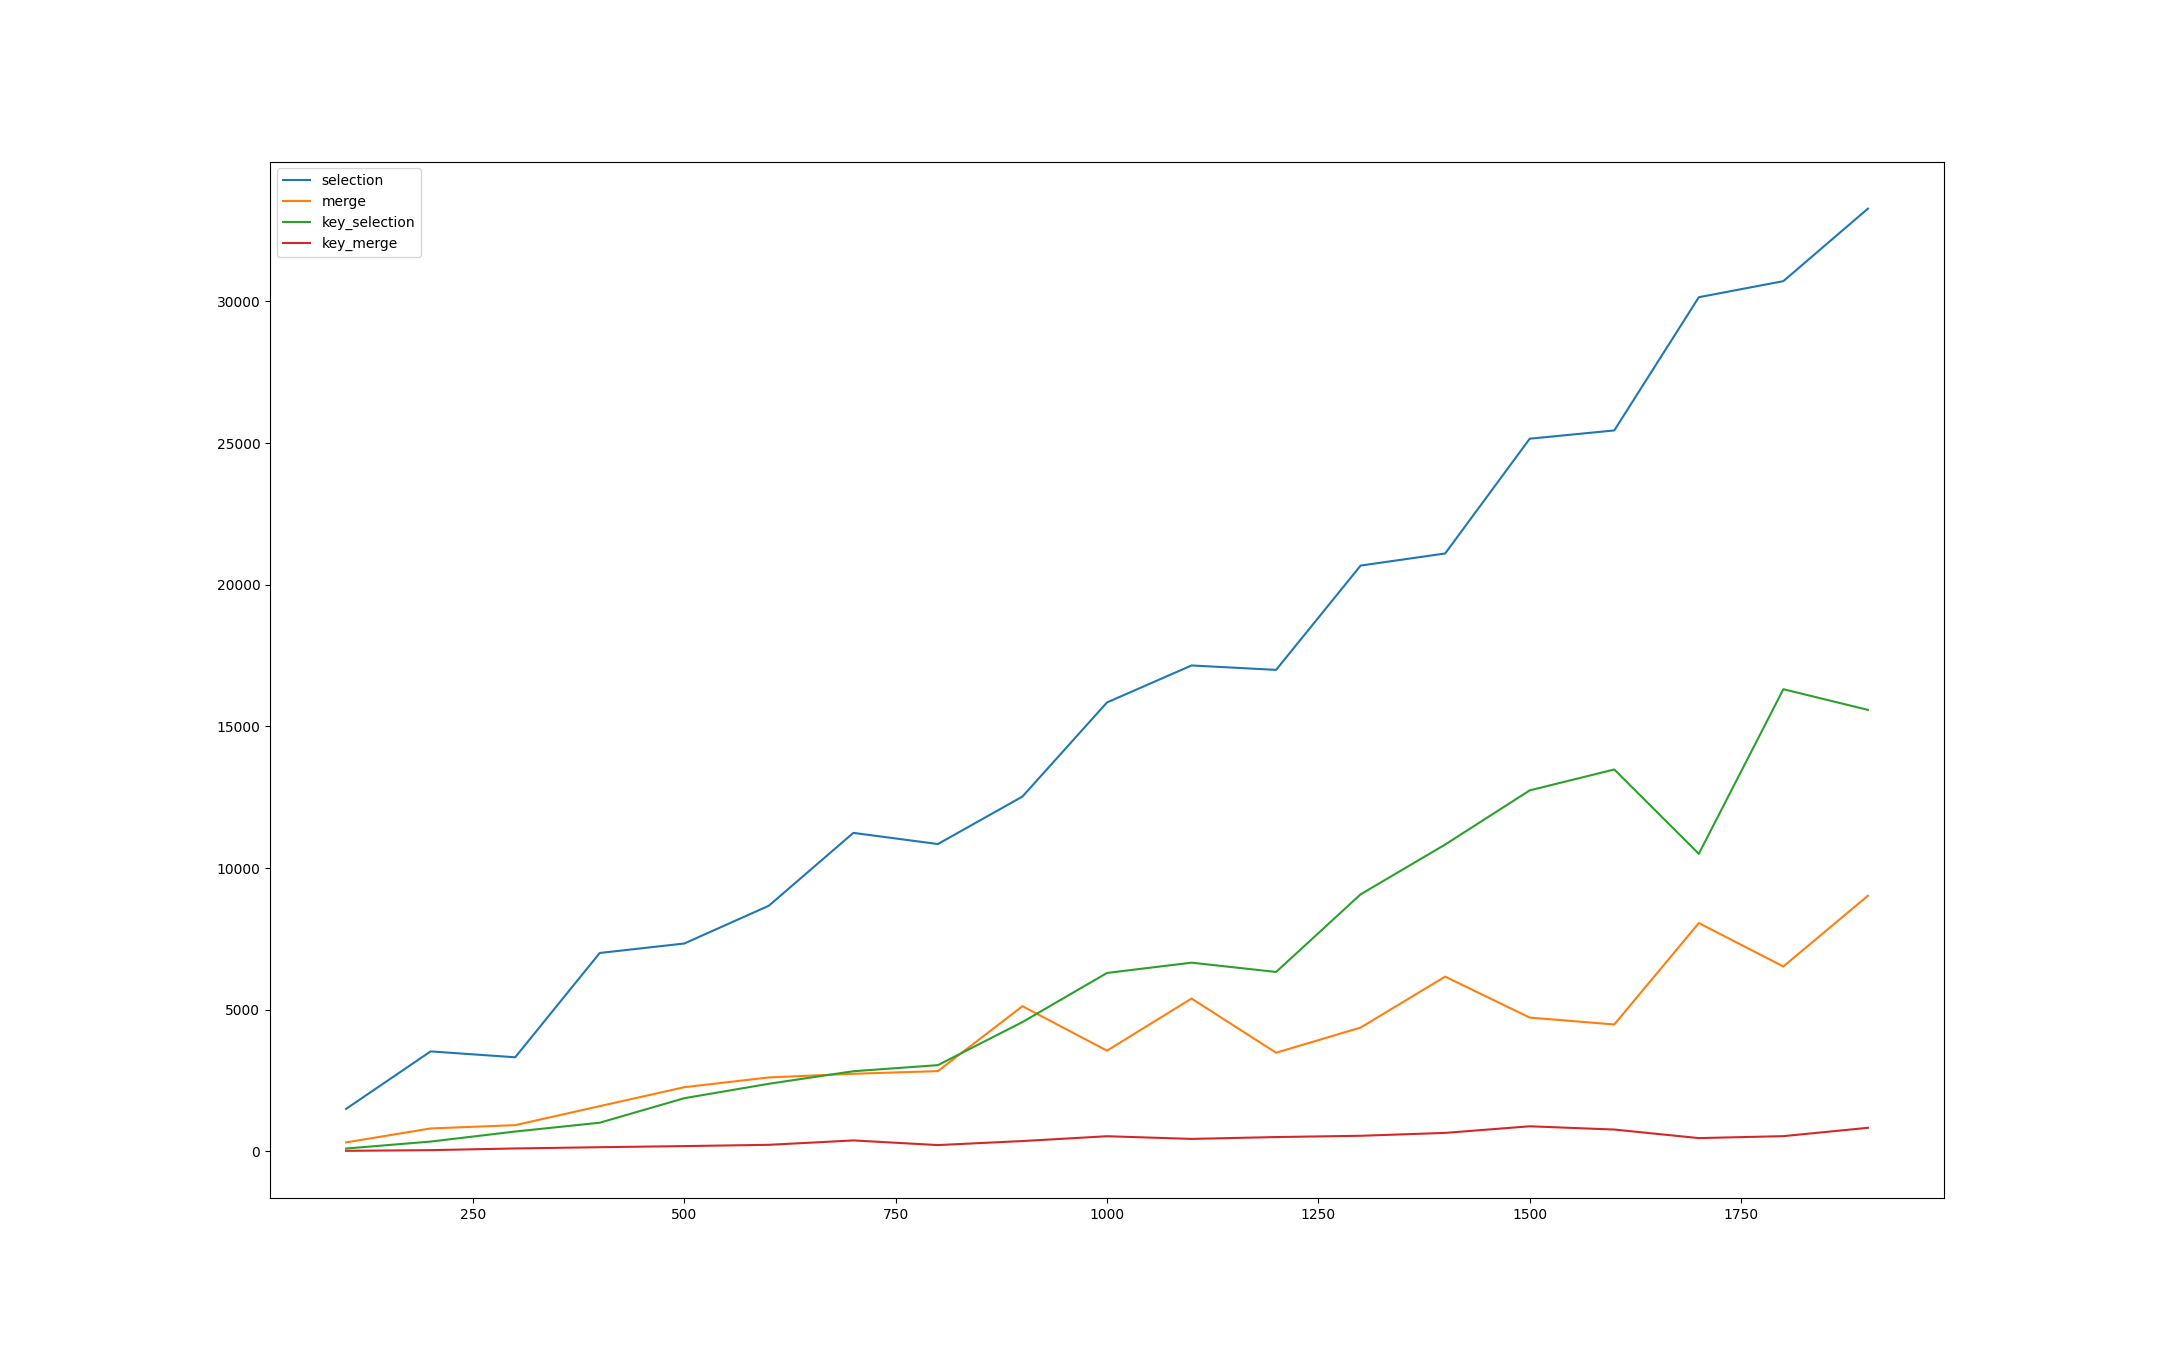
\includegraphics[width=\linewidth]{img/sort_time.png}
	\caption{График зависимости времени выполнения сортировки от размерности сортируемой таблицы}
\end{figure}

\section{Относительная эффективность по времени}

Проведем расчет эффективности по времени изучаемых алгоритмов, согласно формуле (4.1):

\begin{equation}
	f = \frac{t_1 - t_2}{t_1} * 100\%
\end{equation}

\begin{enumerate}
	\item Вставками/слиянием (без ключей) -- 73\%
	\item Вставками/слиянием (с ключами) -- 95\%
	\item С ключами/без ключей (слияние) -- 90\%
	\item С ключами/без ключей (выбором) -- 53\%
\end{enumerate}

\section{Вывод}

Реализация алгоритма сортировки слиянием выполняется примерно в 4 раза быстрее, чем реализации алгоритма сортировки вствками. Сортировка вставками по ключам увеличивает эффективность по времени еще в 10 раз. Таким образом использование таблицы ключей при сортировке больших таблиц увеличивает эффективность по времени, но в то же время требует дополнительных затрат памяти на хранение самой таблицы.

\chapter{Контрольные вопросы}

\begin{enumerate}
	\item Как выделяется память под вариантную часть записи?
	
	Память  под  вариантную  часть  записи  выделяется  единым  блоком, который  по  своему  объему  может  уместить  максимальный  тип  из используемых. При этом остальные типы используют ту же область памяти, 
	из-за чего могут быть логические ошибки при неверном интерпретировании имеющихся в вариантой части данных.
	
	\item Что  будет, если  в  вариантную  часть  ввести  данные,  несоответствующие 
	описанным?
	
	В  лучшем  случае  произойдет  ошибка  компиляции.  В  худшем  — введённые  данные будут неправильно интерпретироваться в дальнейшем и в какой-то момент приведут к более серьёзным последствиям.
	\item Кто  должен  следить  за  правильностью  выполнения  операций  с  вариантной 
	частью записи? 
	
	За правильностью выполнения операций с вариантной частью должен следить сам программист.
	
	\item Что представляет собой таблица ключей, зачем она нужна?
	
	Таблица ключей  представляет собой массив из упрощенных моделей обычных  записей,  которые  включают  в  себя  минимально  возможную информацию для однозначного сопоставления их с исходными записями. 
	Таблица ключей нужна для сокращения времени работы с исходной таблицей при необходимости частой модификации структуры таблицы, но не самих  записей  в  ней.  Например,  такой  модификацией  можно  считать сортировку записей, вставку новой записи с сохранением упорядоченности таблицы.
	
	\item В каких случаях эффективнее обрабатывать данные в самой таблице, а когда – 
	использовать таблицу ключей?
	
	В  случаях,  когда  память  является  более  весомым  критерием эффективности, следует обрабатывать данные непосредственно на месте, а когда на первом месте стоит время, то конечно стоит использовать таблицу ключей. 
	Также, если в самой таблице не очень много данных, и они не часто обрабатываются,  то  перебарщивать  с  оптимизацией не  нужно  — в большинстве  случаев  прирост  производительности  будет  неоправданным (если вообще будет). 
	
	\item Какие способы сортировки предпочтительнее для обработки таблиц и почему?
	
	Для  обработки  таблиц  предпочтительнее  использовать  способы сортировки не требующие большого количества проходов по всему объему данных,  так  как  таблицы  зачастую  хранят  довольно  большие  объемы информации и такие «обходы» могут очень дорого обойтись, когда речь зайдёт об эффективности алгоритмов сортировки.
\end{enumerate}

